\ifx\mainfile\undefined
%  ========================================================================
%  Copyright (c) 2006-2011 The University of Washington
%
%  Licensed under the Apache License, Version 2.0 (the "License");
%  you may not use this file except in compliance with the License.
%  You may obtain a copy of the License at
%
%      http://www.apache.org/licenses/LICENSE-2.0
%
%  Unless required by applicable law or agreed to in writing, software
%  distributed under the License is distributed on an "AS IS" BASIS,
%  WITHOUT WARRANTIES OR CONDITIONS OF ANY KIND, either express or implied.
%  See the License for the specific language governing permissions and
%  limitations under the License.
%  ========================================================================
%
 
\documentclass [11pt, twoside] {uwthesis}

\usepackage{color}
\usepackage{url}
\usepackage{amsmath}
\usepackage{amsfonts}
\usepackage[bookmarks,
	hidelinks,
	plainpages=false,
	pdfpagelabels,
	pagebackref=true,
            ]{hyperref}
\renewcommand*{\backref}[1]{}% for backref < 1.33 necessary
\renewcommand*{\backrefalt}[4]{%
  \ifcase #1 %
    (No citations.)%
  \or
    (Cited on page #2.)%
  \else
    (Cited on pages #2.)%
  \fi
}

\newcommand{\biburl}[1]{{\tt<}\url{#1}{\tt>}}

\hypersetup{%
pdfauthor = {Daniel Chaim Halperin},
pdftitle = {Simplifying the Configuration of 802.11 Wireless Networks with Effective SNR},
pdfsubject = {Ph.D. Dissertation},
pdfkeywords = {},
pdfcreator = {University of Washington, Computer Science and Engineering},
pdfproducer = {},
bookmarksopen = {true},
pdfpagelayout = {TwoColumnRight},
}

\usepackage{footnotebackref}
%%%%%%%%%%%%%%%%%%%%%%%%%%%%%%%%%%%%%%%%%%%%%%%%%%%%%%
%%%        Formatting sections                     %%%
%%%%%%%%%%%%%%%%%%%%%%%%%%%%%%%%%%%%%%%%%%%%%%%%%%%%%%
\newcommand{\algref}[1]{Algorithm~\ref{#1}}
\newcommand{\chapref}[1]{Chapter~\ref{#1}}
\renewcommand{\eqref}[1]{Equation~\ref{#1}}
\newcommand{\figref}[1]{Figure~\ref{#1}}
\newcommand{\secref}[1]{\S\ref{#1}}
\newcommand{\tabref}[1]{Table~\ref{#1}}
\newcommand{\heading}[1]{\vspace{4pt}\noindent\textbf{#1}}
\newcommand{\topheading}[1]{\noindent\textbf{#1}}
\newcommand{\noheading}[0]{\vspace{4pt}\noindent}

%%%%%%%%%%%%%%%%%%%%%%%%%%%%%%%%%%%%%%%%%%%%%%%%%%%%%%
%%%        XXX and other warnings                  %%%
%%%%%%%%%%%%%%%%%%%%%%%%%%%%%%%%%%%%%%%%%%%%%%%%%%%%%%
\newcommand{\xxx}[1]{\textit{\color{red}XXX #1}}

%%%%%%%%%%%%%%%%%%%%%%%%%%%%%%%%%%%%%%%%%%%%%%%%%%%%%%
%%%        Units                                   %%%
%%%%%%%%%%%%%%%%%%%%%%%%%%%%%%%%%%%%%%%%%%%%%%%%%%%%%%
\usepackage{xspace}
\newcommand{\unitsep}{\texorpdfstring{\,}{ }}
\def\unit#1{% from: http://www.tex.ac.uk/cgi-bin/texfaq2html?label=csname "Defining a macro from an argument"
  \expandafter\def\csname #1\endcsname{\unitsep\text{#1}\xspace}%
}
\def\varunit#1#2{% from: http://www.tex.ac.uk/cgi-bin/texfaq2html?label=csname "Defining a macro from an argument"
  \expandafter\def\csname #1\endcsname{\unitsep\text{#2}\xspace}%
}
\unit{GHz}
\unit{MHz}
\unit{kHz}
\unit{Gbps}
\unit{Mbps}
\unit{KB}
\unit{dB}
\unit{dBi}
\unit{dBm}
\unit{W}
\unit{mW}
\varunit{uW}{$\mu$W}
\unit{ms}
\varunit{us}{$\mu$s}
\unit{h}
\unit{m}
\unit{s}
\unit{km}
\unit{cm}
\unit{mm}
\varunit{mmsq}{mm$^\text{2}$}
\varunit{insq}{in$^\text{2}$}
\newcommand{\degree}{\ensuremath{^\circ}\xspace}
\newcommand{\degrees}{\degree}
%%%%%%%%%%%%%%%%%%%%%%%%%%%%%%%%%%%%%%%%%%%%%%%%%%%%%%%%%%%%%%%%%%%%%%%%%%%%%%%%%%%%%%
% Euler for math | Palatino for rm | Helvetica for ss | Courier for tt
%
% From: http://www.tug.org/mactex/fonts/LaTeX_Preamble-Font_Choices.html
%%%%%%%%%%%%%%%%%%%%%%%%%%%%%%%%%%%%%%%%%%%%%%%%%%%%%%%%%%%%%%%%%%%%%%%%%%%%%%%%%%%%%%
\renewcommand{\rmdefault}{ppl} % rm
\usepackage[scaled]{helvet} % ss
\usepackage{courier} % tt
\usepackage{eulervm} % a better implementation of the euler package (not in gwTeX)
\normalfont
\usepackage[T1]{fontenc}
%%%%%%%%%%%%%%%%%%%%%%%%%%%%%%%%%%%%%%%%%%%%%%%%%%%%%%%%%%%%%%%%%%%%%%%%%%%%%%%%%%%%%%

%%%%%%%%%%%%%%%%%%%%%%%%%%%%%%%%%%%%%%%%%%%%%%%%%%%%%%
%%%        Figures                                 %%%
%%%%%%%%%%%%%%%%%%%%%%%%%%%%%%%%%%%%%%%%%%%%%%%%%%%%%%
\usepackage{graphicx}
% Caption package both lets you set the spacing between figure and caption
% and also makes the \figref{} point to the right place.
\usepackage[font=bf,aboveskip=6pt,belowskip=-4mm]{caption}
% Allow subfigures, make them bold
\usepackage[bf,BF,small]{subfigure}
% List of figures
\setcounter{lofdepth}{2}  % Print the chapter and sections to the lot

%%%%%%%%%%%%%%%%%%%%%%%%%%%%%%%%%%%%%%%%%%%%%%%%%%%%%%
%%%        Lists with reduced spacing              %%%
%%%%%%%%%%%%%%%%%%%%%%%%%%%%%%%%%%%%%%%%%%%%%%%%%%%%%%
\usepackage{enumitem}

%%%%%%%%%%%%%%%%%%%%%%%%%%%%%%%%%%%%%%%%%%%%%%%%%%%%%%
%%%        Fancy tables                            %%%
%%%%%%%%%%%%%%%%%%%%%%%%%%%%%%%%%%%%%%%%%%%%%%%%%%%%%%
\usepackage{tabulary}
\usepackage{booktabs}

%%%%%%%%%%%%%%%%%%%%%%%%%%%%%%%%%%%%%%%%%%%%%%%%%%%%%%
%%%        Formatting techniques/tools/etc.        %%%
%%%%%%%%%%%%%%%%%%%%%%%%%%%%%%%%%%%%%%%%%%%%%%%%%%%%%%
\newcommand{\term}[1]{\texttt{#1}}

\begin{document}
 
\textpages
\setcounter{chapter}{1} % Set to n-1!
\fi
%%%%%%%%%%%%%%%%%%%%%%%%%%%%%%%%%%

\cleardoublepage
\chapter{Background}
\label{chap:background}

In this chapter, I establish the fundamentals of wireless communication and the IEEE 802.11 standards to the extent needed to understand my thesis.

\section{Digital Communication Principles}
Electromagnetic (EM) communications, which send data using \define{electromagnetic signals}, form the basis of the technologies I will discuss in this thesis. One key aspect of each wireless technology is which part of the electromagnetic spectrum it uses, characterized by its \define{carrier frequency or center frequency}, denoted $f$. A fundamental property of radio waves is that the frequency of a wave determines its \define{wavelength} $\lambda$ according to the relationship $c=f\lambda$, where $c$ is the speed of light. IEEE~802.11 networks typically use EM signals with a carrier frequency in the range of 2.4\GHz and 5\GHz and corresponding wavelengths of about 12\cm and 6\cm.

Data transmission using EM signals works by \define{modulating} a pure sine wave with frequency $f$, i.e.\ by transforming the sine wave to reflect the underlying data. The simplest modulation scheme might be to turn the sine wave on or off depending on whether the bit to be transmitted is a 1 or a 0. The rate at which the transmitter varies the signal---in this example, the rate the sine wave is turned on or off---is called the \define{symbol rate}, and determines the \emph{bandwidth} of the channel $B$ measured in Hertz (Hz).

The \emph{amplitude} of the sine wave, e.g. how much the peak varies from the zero (usually measured in volts (V)), determines the \define{power} of the signal. These two quantities are related by a quadratic relationship: doubling the amplitude of a signal results in a quadrupling of the signal power.

In a \define{link}, that is a sender communicating data to a receiver, the sender generates a signal with \define{transmit (signal) power} level $T$ that propagates through the \define{channel} connecting the two. The channel could be a \define{wire} or it could be the free-space \define{radio frequency (RF)} environment in which signals propagate from the transmitter's antenna to the receiver's antenna over the air.

\subsection{The Wired Channel}
To simplify the discussion, I will start with the case of a wired channel. The transmitted signal propagates down the wire to the receiver and then is received with \define{receive (signal) power} $S$. While propagating through the wire, the signal gets slightly weaker as a small amount of energy is absorbed. The net effect of this absorption is called \define{attenuation}, denoted $\alpha$, and is defined mathematically as the multiplicative decrease in power induced by the channel:
\begin{equation}
	\label{eq:attenuation}
	\alpha = \frac{T}{S}.
\end{equation}
In addition to attenuation, the wired channel also induces a \define{phase shift} as the electromagnetic signal propagates. The value of this phase shift, denoted $\theta$, depends on factors including the length of the wire and the frequency of the signal, and is generally considered to be an unknown, uniformly random quantity between $0$ and $2\pi$.

\begin{table}
\centering
\begin{tabular}{cll}
\toprule%
Variable & Meaning & Units\\
\midrule%
$f$ & Frequency & Hz \\
$\lambda$ & Wavelength & m \\
$B$ & Bandwidth & Hz \\
$T$ & Transmit signal power & dBm (decibels relative to 1 milli-Watt) \\
$S$ & Receive signal power & dBm \\
$\alpha$ & Attenuation & dB (decibels, unitless) \\
$\theta$ & Phase & radians \\
$N$ & Noise power & dBm \\
$K$ & Temperature & kelvins \\
$\rho$ & Signal-to-noise ratio (SNR) & dB \\
$R$ & Shannon Capacity & bits \\
$d$ & Distance & m \\
$n$ & Path loss exponent & unitless \\
$I$ & Interference power & dBm \\
$\rho_I$ & SINR & dB \\
$M$ & Number of transmit antennas & (antennas) \\
$N$ & Number of receive antennas & (antennas)\\
\bottomrule
\end{tabular}
\caption[Table of notation used in this chapter]{\label{tab:bg_notation}Table of notation used in this chapter.}
\end{table}

The signal measured by the receiver is also corrupted by broad-spectrum electromagnetic noise. This corruption is sometimes called \define{Johnson-Nyquist noise} after its identification in 1927 by Johnson~\cite{Johnson_noise} and explanation in 1928 by Nyquist~\cite{Nyquist_noise}, but it is more commonly known as \define{thermal noise}. Thermal noise can be modeled as a complex Gaussian with average \define{noise power} $N$ (in Watts) equal to
\begin{equation}
\label{eq:noise}
N = kKB,
\end{equation}
where $k\approx1.38\times10^{-23}$ (in Joules/kelvin) is Boltzmann's constant, $K$ is the temperature (in kelvins), and $B$ is the bandwidth. This is called additive, white Gaussian noise (AWGN).
%For a device at room temperature ($\approx$ 293\K), we can compute $N$ in dBm using the approximation
%\begin{equation}
%N \text{ (dBm)} = -174 + 10\log_{10}(B).
%\end{equation}

In the context of 802.11, we typically measure power-related quantities on a logarithmic scale to capture the wide range of possible values. Power levels such as the quantities $T$, $S$, and $N$ are usually measured in decibels relative to 1~milliwatt, or dBm, and typically take on values like $T=20\dBm$ (100\mW) and $S=-80\dBm$ ($10^{-8}$\mW or 10\pW). To calculate $N$, we can use \eqref{eq:noise}: Wi-Fi links typically use bandwidths $B$ of 20\MHz or 40\MHz, which correspond to thermal noise levels of $-$101\dBm and $-$98\dBm at room temperature. In practice, the total noise is assumed to be thermal noise plus a 5\dB--15\dB \define{noise figure}, which is a quantity that estimates additional error added by imperfect analog hardware used in receiver processing. The total noise for a 20\MHz Wi-Fi channel might then be in the range of $-91$\dBm.

Now that we have defined the signal and noise powers, we can discuss the limits of the communication channel. In their seminal works, Ralph Hartley~\cite{Hartley_law} and Claude Shannon~\cite{Shannon_coding,Shannon_capacity} proved that the \define{capacity} of a channel---i.e., the maximum data rate $R$ at which the transmitter and receiver can communicate---is determined by the channel's bandwidth and its \define{signal-to-noise ratio (SNR)}. The SNR, denoted by $\rho$, is a unitless quantity typically measured in decibels and calculated as
\begin{equation}
\rho = \frac{S}{N}.
\end{equation}
For the example signal power of $-80\dBm$ and noise power of $-91\dBm$, this corresponds to an SNR of $11\dB$.


The Shannon-Hartley Theorem~\cite{Shannon_capacity} establishes what is called the \define{Shannon capacity} to be
\begin{equation}
\label{eq:shannon_capacity}
R = B\log_2(1+\rho).
\end{equation}
\figref{fig:shannon} shows this relationship for the normalized quantity $R/B$.

\begin{figure}[tb]
\centering
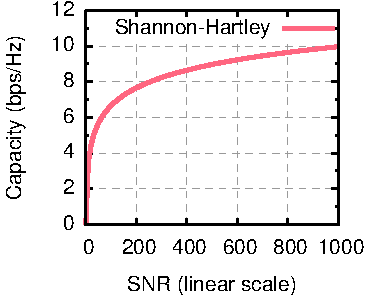
\includegraphics{calculations/shannon}\hspace{0.65in}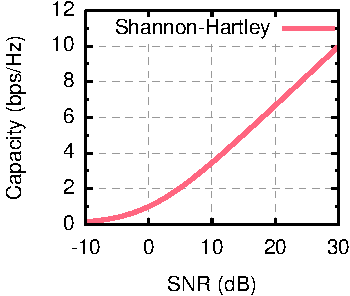
\includegraphics{calculations/shannon_log}\hspace{0.1in}
\caption[The Shannon Capacity of a communications channel with Gaussian noise]{\label{fig:shannon}The Shannon Capacity of a communications channel with Gaussian noise, presented in both linear and logarithmic (dB) scales.}
\end{figure}

The Shannon-Hartley Theorem determines a bound on the maximum rate achievable as a function of the bandwidth and signal strength. However, it does not give a practical scheme that realizes this bound, and instead systems like 802.11 use many different modulations that achieve different points along the $y$-axis, and choose among these in practice depending on the underlying channel conditions.

Note that for real links, the values of $S$ and $N$ are not known a priori. Instead, transmitters choose an encoding, and the receiver will be able to decode it successfully if the choice falls below the curve for the SNR experienced. The general problem of choosing the modulation to use, as well as the selection of other physical layer parameters, is the focus of my thesis. I describe this problem in more detail in the next chapter.

The binary modulation system I discussed above is a scheme called On-Off Keying~(OOK\@). Each symbol conveys 1 bit, and since the symbol rate is directly tied to the bandwidth used by a scheme, OOK can deliver at most 1 bps/Hz. A generalized form of OOK is Amplitude Shift Keying~(ASK\@), which can send more bits per symbol using multiple power levels. $m$-ASK, i.e., ASK with $m$ power levels per symbol, can deliver up to $\log_2(m)$ bits per symbol and thus can achieve a higher capacity.

\begin{figure}[t]
\centering
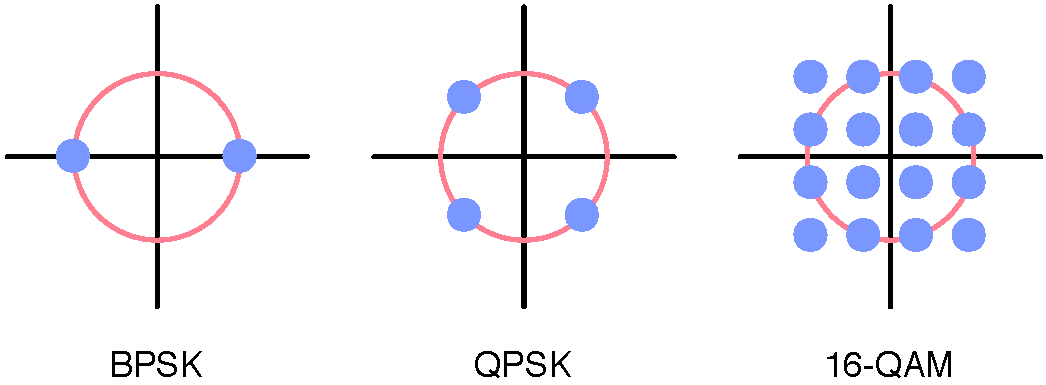
\includegraphics[width=0.9\textwidth]{figures/constellations_radius}
\caption[Constellation diagrams for the BPSK, QPSK, and 16-QAM modulations]{\label{fig:constellations}Constellation diagrams for the BPSK, QPSK, and 16-QAM modulations. These constellations are normalized such that each modulation has equal average transmit power, indicated by the red circle.}
\end{figure}

As mentioned above, electromagnetic signals actually have both an amplitude and a phase. Amplitude modulation varies one of these parameters, and a complementary scheme called Phase-Shift Keying~(PSK) keeps the amplitude constant but varies the phase. A third scheme known as Quadrature Amplitude Modulation~(QAM) varies both parameters simultaneously and results in a more efficient system when sending more than 2 bits per symbol. Noting that the polar coordinates given by amplitude and phase can equivalently be thought of as a complex number, $m$-QAM can be equivalently thought of as $\sqrt{m}$-ASK in both the real and complex dimensions simultaneously. \figref{fig:constellations} shows the two-dimensional \define{constellations} that result from picturing the symbols sent in BPSK (i.e.\ 2-PSK), QPSK (i.e.\ 4-PSK), and 16-QAM modulation schemes.

There are many more modulation schemes than I have presented here, but PSK and QAM are the modulations applicable to 802.11.
%Currently, Wi-Fi devices transmit data using 2-PSK (called Binary PSK, or BPSK), 4-PSK (called Quadrature PSK\@, or QPSK\@), 16-QAM\@, or 64-QAM\@.
64-QAM is the highest modulation currently used by Wi-Fi devices, though the future IEEE 802.11ac amendment~\cite{80211ac} will add 256-QAM to this set.

Recall that the signal will be corrupted by noise when measured at the receiver. Under the standard AWGN model, we model this corruption as shifting the received symbol by a random complex vector whose length depends on the noise power. We see in \figref{fig:constellations} that the different modulations have different constellation densities: the symbols of 16-QAM are clustered more closely than the symbols of QPSK or BPSK. This means that higher constellations which encode more bits per symbol are more vulnerable to noise. At low SNR, the receiver cannot easily distinguish between many symbols, so slower modulations with fewer constellation points should be used. At high SNR, the receiver can distinguish between more symbols and thus can use a denser constellation.

\begin{figure}[t]
\centering
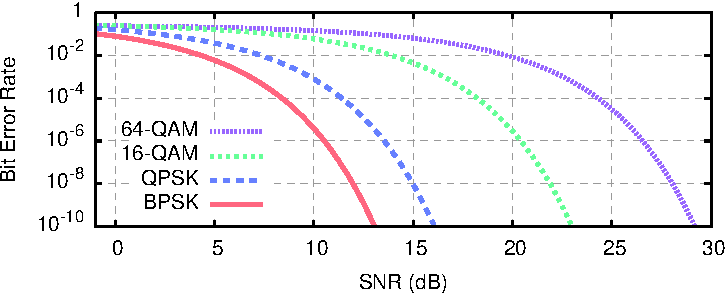
\includegraphics{calculations/snr_ber}
\caption[BER vs SNR for the four 802.11n modulation schemes]{\label{fig:mod_ber_snr}The relationship between bit error rate and SNR for the four 802.11 modulation schemes.}
\end{figure}

\begin{figure}[t]
\centering
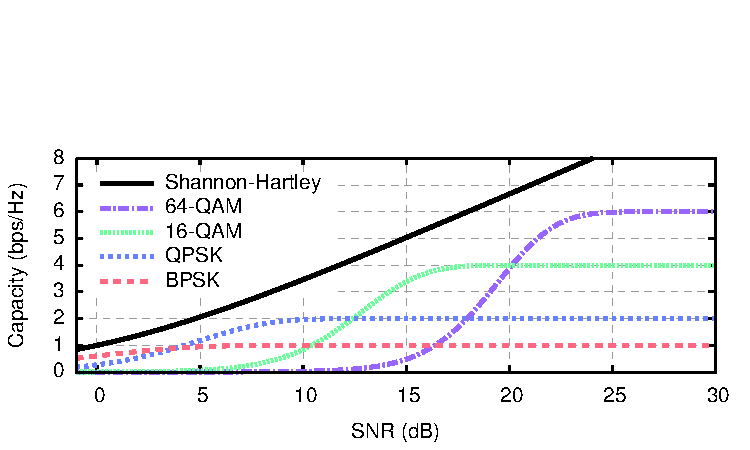
\includegraphics{calculations/snr_bits}
\caption[Capacity vs SNR for 802.11n modulation and coding schemes]{\label{fig:mod_bits_snr}The relationship between SNR and capacity for standard modulation schemes and idealized codes.}
\end{figure}

This property of the performance of different modulation schemes is closely related to the Shannon Capacity. \figref{fig:mod_ber_snr} illustrates the magnitude of this effect for the modulations used by 802.11 using textbook formulas~\cite{Sklar} that relate the SNR to a bit error rate. We can also connect these different modulations directly to the Shannon-Hartley Capacity Theorem by examining the capacity achieved by each scheme as a function of SNR (\figref{fig:mod_bits_snr}). In this graph, I assume an idealized coding scheme that delivers the maximum data rate for a given bit error rate; the practical schemes in widespread use today are somewhat less efficient in order to admit less expensive computation.\footnote{Though beyond the scope of this thesis, a number of recent proposals for practical \define{rateless codes}~\cite{Gudipati_Strider,Perry_Spinal} nearly achieve the Shannon Capacity bound by using much denser constellations and clever coding schemes across multiple transmissions.}

\subsection{The Wireless Channel}
The previous section explained the basics of digital communications in the context of a wired link. Here, I expand to the significantly more complex case of a wireless channel.

In a wireless link, the electromagnetic signal is emitted from an antenna as a \define{radio wave} that then radiates through the \define{wireless medium}, i.e.\ the environment. The dominant source of attenuation in an wireless link is not absorption by the medium, but rather the diffusion of energy throughout the environment, of which a small fraction is captured by a receiver's antenna. This effect, called \define{path loss}, is captured by the Friis transmission equation, which yields the inverse relationship
\begin{equation}
\label{eq:friis}
	S \propto \frac{T}{d^n},
\end{equation}
where $d$ is the distance between transmitter and receiver, and $n$ is the path loss exponent. In free space, $n$ has a value of 2, reflecting the fact that the energy transmitted at a particular time is spread out over the two-dimensional surface of a sphere, an area that grows with $d^2$. (For a directional antenna, the energy is spread over a different geometric shape, e.g. a cone, but this shape will still have a two-dimensional surface area).

The path loss exponent varies in different indoor environments, but empirically tends to take on a value between 2 and 4~\cite{Sklar}. This empirical result is explained as the sum of many complex effects that result from the interaction of radio waves with objects in the environment. One such effect is \define{shadowing}, in which materials such as glass or metal prevent radio waves from passing through. I explain more additional, more complicated channel effects below.

In wireless systems, multiple devices might send at the same time and in the same frequency band; this \define{interference} causes a \define{collision} during which a receiver will measure the sum of both transmissions. There are a number of practical problems for operation during a collision, such as whether the receiver can properly lock onto the desired signal and estimate the effects of the channel on it. In general, however, we can model the reception probability by replacing the SNR with the \define{signal-to-interference-and-noise ratio (SINR)}, which treats the interfering signal of power $I$ as another source of noise:
\begin{equation}
\label{eq:sinr}
\rho_I = \frac{S}{I+N}.
\end{equation}
While interference is an important problem, many systems, including 802.11, use \define{medium access control (MAC)} protocols to ensure that at most one device transmit at a time.

Beyond path loss, the most important channel effect is the inherent \emph{multi-path} nature of indoor wireless environments. At 2.4\GHz and 5\GHz, RF signals bounce off metal and glass surfaces that are common indoors. This scattering leads to a situation in which many copies of the signal arrive at the receiver having traveled along many different paths. The net effect of this RF superposition depends on the phases of the individual signals. When these copies combine they may add constructively, giving a good overall signal, or destructively, mostly canceling the overall signal.

The phase-dependent nature of multi-path effects means that they vary over both frequency and space. For a given distance traveled $d$, the phase change is $2\pi d/\lambda$. Thus wideband channels may exhibit dramatically different received power levels for different frequencies; such channels are called \define{frequency selective}. Measurement studies of frequency-selective fading report signal variations as high as 15--20\dB~\cite{Judd_CHARM}; in \chapref{chap:problem} I will present experimental evidence confirming these effects in the environments I studied.

With regard to spatial variation, the small 12\cm and 6\cm wavelengths of Wi-Fi signals means that small changes in path lengths can alter a situation from good to bad. Statistical models tell us that multi-path fading effects are independent for locations separated by as little as half a wavelength. This means that multi-path causes rapid signal changes or fast fading as the receiver moves, or in the case of a stationary node as the surrounding environment changes.  Movement at fast speed also induces \define{Doppler effect}, which aggravates multi-path effects and makes the channel even more variable.
%This means that some unlucky frequencies in a wide channel may be wiped out while others are unaffected.

The net effect of multi-path fading is that the received wireless signal can vary significantly over time, frequency and space. This is a problem for good performance because at any given time there is a significant probability of a deep fade that will reduce the SNR of the channel below the level needed for a given communication scheme.

However, an alternative way of looking at the effects of multi-path fading is that they provide \define{diversity}. In a sufficiently rich multi-path environment, there are so many combining copies of signals that the channel observed on different, nearby frequencies can be considered to be independently faded. For this reason among others, many systems including 802.11 use a scheme called Orthogonal Frequency Division Multiplexing (OFDM). In OFDM, a wide frequency band is split into many \define{subcarriers} that each carry different modulated bits in parallel, with a higher level error-correcting code across them to take advantage of this \define{frequency diversity}.

To get fast rates while only using sending a single symbol at a time, a wideband system must have a fast symbol rate. Since OFDM sends many symbols in parallel on smaller subcarriers, an OFDM system sends each symbol for a longer period of time. Thus by turning a single fast channel into many parallel slower channels, OFDM allows more time for the channel to average out temporal fades and provides \define{time diversity}.

One more type of diversity is \emph{spatial diversity}: antennas separated by at least half a wavelength see independently-faded channels. Devices with multiple antennas can use schemes that take advantage of the spatial diversity these antennas provide. For example, a multi-antenna receiver measures multiple independent copies of each transmitted signal. Thus with clever signal processing, such a receiver can align the phases of these copies and add them together, which averages out the noise and improves overall channel performance. In a complementary manner, a multi-antenna transmitter with knowledge of the fading properties of the individual paths between pairs of antennas can steer its signal such that the multiple copies arriving at the receiver's antenna combine optimally. This process, in which the gain and phase of the signal emitted by each antenna are adjusted (with OFDM, this adjustment may be different for each subcarrier) is called \define{beamforming}.
%A different technique called \define{space-time codes} to achieve the same effect, but 

Finally, suppose that both the transmitter and receiver have multiple antennas. The foundational work by Foschini, Gans~\cite{Foschini_Gans} and Telatar~\cite{Telatar_MIMO} in the mid 1990s introduced \define{spatial multiplexing}, which uses this new spatial degree of freedom to improve capacity. Instead of sending the same data out each antenna as above, a transmitter with $M$ antennas can use its different antennas to send up to $M$ independent \define{spatial streams} of data. An $N$-antenna receiver will then measure $N$ copies of each stream, each antenna an independent linear combination of the $M$ transmitted streams. If $M \leq N$, the receiver has enough information to solve the linear system and separate the streams, thus providing an $M$-fold gain in performance. Thus spatial multiplexing, with $N$ antennas at each side, results in a modified capacity theorem:
\begin{equation}
\label{eq:mimo_capacity}
R = BN\log_2(1+\rho).
\end{equation}
Together, spatial diversity and spatial multiplexing techniques form a set of what are called MIMO (multiple-input, multiple-output) techniques.

I conclude this discussion by mentioning one last channel effect relevant to 802.11: \define{inter-symbol interference}. In multi-path environments, some spatial paths can be so long that the delayed copies of the signal substantially overlap with the next symbol and make it harder to receive. The delay between the earliest and latest copies is called the \define{delay spread} of the channel, and it can be substantial. OFDM systems that use longer symbol times are more resilient to this effect, but still repeat each symbol for a period of time called a \define{guard interval}. If the guard interval is at least as long as the delay spread, the receiver can ignore the inter-symbol interference and still receive a complete symbol.

%For a variety of practical reasons, but in large part to combat multi-path fading, many modern protocols use .
%In 802.11, the 20\MHz-wide channel is broken into 64 \define{subcarriers}, each using 312.5\kHz of bandwidth.
%The beauty of OFDM is that it divides the channel in a way that is both computationally and spectrally efficient. High aggregate data rates can be achieved, while the encoding and decoding on different subcarriers can use shared hardware components.
%The individual subcarriers yield relatively independently faded channels (because of multi-path fading), and hence provide \define{frequency diversity} that is realized by coding across them.

%Dividing the channel also increases the symbol time per channel, since many slow symbols are sent in parallel instead of many fast symbols in sequence. This adds \define{time diversity} because the channel is more likely to average out fades over a longer period of time. Additionally, OFDM links compensate for multi-path by 
%In 802.11, which is targeted for roughly 100\m links, a secondary path might travel 200\m before reflecting, delayed by 667\ns from a pure line-of-sight path; 802.11 uses an 800\ns guard interval to compensate.  

%\begin{itemize}
%\item Fading, multipath, Doppler, etc. All of the above describe how we can get capacity out of the wireless channel. The hard part, and what most of all Wi-Fi research centers around, is how we develop protocols and systems to realize this capacity in the face of these effects.

%\item Collisions and SINR.

%\end{itemize}

\subsection{Summary}
\label{sec:background_80211n}
In this section, I have presented the fundamental principles of digital communication of wired and wireless channels, including the limits of noisy RF channels and how data is encoded. I have also described the most relevant channel effects that communicating devices must overcome, and the primary techniques used to do so. In the next section, I make this discussion concrete in the context of Wi-Fi by describing the specifics of the IEEE 802.11n standard. 

\section{The IEEE 802.11n Standard}
The IEEE 802.11 (Wi-Fi) standard~\cite{80211} is targeted towards defining a mode of operation for a \define{wireless local area network (WLAN)}, intended to provide medium-range connectivity ($\approx$100\m) using low transmit power (at most 1\W). It was first introduced in 1997, and has been amended many times since. In this thesis, I limit my discussion to the features of 802.11n, the newest physical layer amendment, and 802.11a, its predecessor.

Wi-Fi devices use unlicensed spectrum in the 2.4\GHz and 5\GHz bands, and must coexist with consumer electronics such as microwaves, cordless phones, and baby monitors. In addition to this cross-device interference, nearby Wi-Fi networks in separate administrative domains---such as neighboring apartments---may need to share the same channel. As a result, Wi-Fi networks are not planned in a centralized fashion, but rather use decentralized protocols that work towards a good solution in a distributed fashion. For instance, 802.11 includes a \define{carrier-sense multiple access (CSMA)} protocol to manage which devices send: in essence, a transmitter listens to ensure no other devices are transmitting before sending a packet, and reduces its sending probability exponentially (via \define{exponential backoff}) if its transmission is not acknowledged.

At the physical layer, 802.11 uses the modulation schemes and OFDM I described above, operating over 20\MHz channels. In conjunction with different modulations, 802.11 also uses error-correcting codes with different \define{coding rates} to achieve different operating points in the rate-robustness tradeoff space. I summarize the specific single-stream configurations in 802.11n as well as the resulting link data rates in \tabref{tab:siso_mcs}.

\begin{table}[t]
\centering
%\footnotesize
\begin{tabular}{cccc}
\toprule
MCS & Modulation & Coding Rate & Data Rate (Mbps) \\
\midrule
0 & BPSK & 1/2 & 6.5 \\
1 & QPSK & 1/2 & 13.0\\
2 & QPSK & 3/4 & 19.5\\
3 & 16-QAM & 1/2 & 26.0\\
4 & 16-QAM & 3/4 & 39.0\\
5 & 64-QAM & 2/3 & 52.0\\
6 & 64-QAM & 3/4 & 58.5\\
7 & 64-QAM & 5/6 & 65.0\\
\bottomrule
\end{tabular}
\caption[The 802.11n single-stream rates]{\label{tab:siso_mcs} The single-stream 802.11n modulation and coding schemes (MCS). These are only slightly different than the 802.11a MCS that achieved up to 54\Mbps. The increase in maximum rate comes from slightly more efficient use of OFDM subcarriers and a new, less redundant 5/6-rate code.}
\end{table}

The standard link metric is the \define{receive signal strength indicator (RSSI)}. The RSSI was included in the 802.11 standard from the beginning as ``a measure by the [physical layer hardware] of the energy observed at the antenna used to receive the current [packet]''~\cite[\S 17.2.3.2]{80211}. There are no specified requirements on its accuracy, instead, it is only required to be ``a monotonically increasing function of the received power''~\cite[\S 17.2.3.2]{80211}, and is generally used by the hardware to tell whether another device is transmitting. In practice, however, the RSSI reported by commercial Wi-Fi chipsets is an estimate of the received signal power and can be meaningfully translated into units of dBm. In this case, RSSI can be used in combination with noise measurements to compute the SNR of the link.

The 2009 standard amendment to IEEE 802.11n~\cite{80211n} added functionality and protocols for multi-antenna techniques such as spatial diversity, spatial multiplexing, and beamforming. The 802.11n enhancements are shown in \tabref{tab:11n_enhancements}. Most of improvement in the maximum data rate---from 54\Mbps in 802.11a to 600\Mbps in 802.11n---comes from the ability to use wider channels and multiple spatial streams. Together, these add $2\cdot2\cdot4=16$ times as many configurations to the space of a single link. Beamforming is effectively an analog parameter and adds nearly unbounded options.\footnote{For transmitter and receiver each using 4 antennas on a 40\MHz channel, representing the beamforming matrices at maximal resolution takes 29,184 bits.} The gains of beamforming vary depending on the channel---for strong links, they tend to be small, but for weak links they can provide dramatic performance improvements~\cite{Atheros_11nTechPaper}.

\begin{table}[t]
\centering
%\footnotesize
\begin{tabular}{lcp{3.1in}}
\toprule
Enhancement & Capacity Gain & Description \\
\midrule
Short OFDM & \multirow{2}{*}{$1.11\times$} & Data can be more efficiently encoded when the \\
guard interval & & multi-path delay spread is low.\\
\multirow{2}{*}{Spatial multiplexing} & \multirow{2}{*}{$2\times$ to $4\times$} & \multirow{2}{*}{Up to 4 concurrent spatial streams.} \\
\vspace{-6pt}\\
\multirow{2}{*}{40\MHz channels} & \multirow{2}{*}{$2.08\times$} & \multirow{2}{*}{More bandwidth, higher capacity (\sheqref{eq:shannon_capacity}).} \\
\\
\multirow{3}{*}{Beamforming} & \multirow{3}{*}{??} & A sender with multiple transmit antennas can shape its signal to match the RF channel, improving both performance and reliability. \\
\bottomrule
\end{tabular}
\caption[The 802.11n physical layer enhancements]{\label{tab:11n_enhancements} IEEE~802.11n adds a number of enhancements to the base single-stream configurations depicted in \tabref{tab:siso_mcs}. The performance improvement from beamforming varies depending on the properties of the wireless channel.}
\end{table}

The hardware/software interface in 802.11n operates at the level of individual packets or continuously-transmitted batches of packets. Packets are sent to the hardware and transmitted over the air. The receiver detects a new transmission from the increase in energy, estimates the parameters of the wireless channel from the packet's standard, known preamble, and then decodes the packet. The standard behavior for 802.11 links is that all bits---after error correction---must be correct in order for a packet to be received, otherwise the packet is dropped by the hardware. Correctly received packets are delivered to the software layer in conjunction with physical layer configuration information about the transmission (e.g., what MCS in \tabref{tab:siso_mcs} was used) and reception (e.g., which receive antennas were used) of the packet, plus physical layer metrics of link quality.

\section{Summary}
In this chapter, I have presented the background information to provide a basic understanding of wireless channels and the specific IEEE 802.11n technology used to operate in them. As I described in \secref{sec:background_80211n}, there are many different techniques that a transmitter and/or receiver can use to achieve robust operation in indoor wireless channels. However, the challenge---and the focus of most Wi-Fi research---is to decide which techniques to use, when to use them, and how to configure them to obtain the best operating point given the actual properties of the wireless channel. This is the primary problem I tackle in this thesis; in the next chapter I describe this problem in detail and given an overview of my approach.

%%%%%%%%%%%%%%%%%%%%%%%%%%%%%%%%%%
\ifx\mainfile\undefined
%
% ==========   Bibliography   ==========
%
%\nocite{*}   % include everything in the uwthesis.bib file
\bibliographystyle{plain}
\bibliography{dhalperi_thesis}

\end{document}
\fi
